%% Overleaf			
%% Software Manual and Technical Document Template	
%% 									
%% This provides an example of a software manual created in Overleaf.

\documentclass{../ol-softwaremanual}

% Packages used in this example
\usepackage{graphicx}  % for including images
\usepackage{microtype} % for typographical enhancements
\usepackage{minted}    % for code listings
\usepackage{amsmath}   % for equations and mathematics
\setminted{style=friendly,fontsize=\small}
\renewcommand{\listoflistingscaption}{List of Code Listings}
\usepackage{hyperref}  % for hyperlinks
\usepackage[a4paper,top=4.2cm,bottom=4.2cm,left=3.5cm,right=3.5cm]{geometry} % for setting page size and margins

\usepackage[english, greek]{babel}

\usepackage{subfig}


% Custom macros used in this example document
\newcommand{\doclink}[2]{\href{#1}{#2}\footnote{\url{#1}}}
\newcommand{\cs}[1]{\texttt{\textbackslash #1}}

\begin{document}
	
	
	\begin{titlepage}
		
		
		% Frontmatter data; appears on title page
		\title{\en Project Description \\}
		\version{0.1}
		\softwarelogo{
\includegraphics[scale=0.4]{../CarBazaar_logo.png}}
	\end{titlepage}
	
	
	\maketitle
	
	\newpage
	
	\center{\textbf{Μέλη Ομάδας}}
	
	\vspace{60pt}
	
	
	
	\begin{table}[htbp!]
		\begin{tabular}{llll}
			Μεμελετζόγλου Χαρίλαος & 1069364 & \en st1069364@ceid.upatras.gr  & \gr 4ο έτος \\ 
			\\ Λέκκας Γεώργιος      &      1067430    &   \en st1067430@ceid.upatras.gr  & \gr 4ο έτος \\
			\\ Γιαννουλάκης Ανδρέας        &   1067387       & \en st1067387@ceid.upatras.gr  & \gr 4ο έτος         \\
			\\ Κανελλόπουλος Ιωακείμ        &  1070914        &    \en st1070914@ceid.upatras.gr     & \gr 4ο έτος   \\ 
		\end{tabular}
	\end{table}
	
	\center{\textbf{Υπεύθυνοι Παρόντος Τεχνικού Κειμένου}}
	
	\vspace{40pt}
	
	\begin{table}[htbp!]
		\begin{tabular}{ll}
			Μεμελετζόγλου Χαρίλαος & \en Editor \\
			\\ Λέκκας Γεώργιος      &   \en  Editor \\
			\\ Γιαννουλάκης Ανδρέας & \en Peer Reviewer \\
			\\ Κανελλόπουλος Ιωακείμ & \en Peer Reviewer
		\end{tabular}
	\end{table}
	
	
	\vspace{40pt}
	
	\center{\textbf{Εργαλεία που χρησιμοποιήθηκαν}}
	
	\vspace{20pt}
	
	Χρησιμοποιήθηκε το \en \doclink{https://www.overleaf.com/}{Overleaf} \gr για την συγγραφή του \LaTeX\ κώδικα. \break
	
	Για την δημιουργία του λογότυπου, χρησιμοποιήθηκε το εργαλείο \en \doclink{https://www.adobe.com/express/create/logo}{Adobe Express} . \gr
	
	Για την επικοινωνία των μελών της ομάδας, χρησιμοποιείται το \en \doclink{ https://www.discord.com/}{Discord} \gr . \\
	
	
	\newpage
	
	\center{\textbf{Περιγραφή Έργου}} 
	
	\vspace{60pt}
	
	\flushleft
	
	To \en {\textbf{CarBazaar}} \gr είναι μια εφαρμογή μέσω της οποίας διεξάγονται αγοραπωλησίες αυτοκινήτων. \hfill \break
	
	Συγκεκριμένα, ο χρήστης μπορεί να αναζητήσει αυτοκίνητα είτε με βάση τον τίτλο του μοντέλου είτε με βάση την μάρκα, το έτος κυκλοφορίας κλπ, αλλά και να αποθηκεύσει αυτοκίνητα της αρέσκειάς του σε μια \en wishlist \gr, επιτρέποντας, έτσι, στην εφαρμογή να του προτείνει παρόμοια αυτοκίνητα στο μέλλον.
	Ακόμη, υπάρχει δυνατότητα να δημιουργήσει μια αγγελία πώλησης ενός δικού του οχήματος αλλά και να δει αγγελίες οχημάτων αναρτημένες από άλλους χρήστες.
	Τέλος, με βάση την τοποθεσία του χρήστη, η εφαρμογή μπορεί να εντοπίσει κοντινές αντιπροσωπείες οχημάτων. \hfill \break
	
	Στην πλατφόρμα, πωλούνται και μεταχειρισμένα αλλά και καινούρια αυτοκίνητα. Στην πρώτη περίπτωση, ο πωλητής μπορεί να είναι είτε ιδιώτης είτε μια αντιπροσωπεία, ενώ στην δεύτερη περίπτωση, ο πωλητής είναι αποκλειστικά και μόνο μια αντιπροσωπεία. \hfill \break
	
	Επίσης, συμμετέχουν και ελεγκτές οι οποίοι μπορούν να μισθωθούν από τον χρήστη, με σκοπό τον έλεγχο της κατάστασης του οχήματος το οποίο ενδιαφέρεται να αγοράσει ο χρήστης. \hfill \break
	
	Ακόμα, υπάρχει η δυνατότητα μεταφοράς ενός οχήματος στην περιοχή του αγοραστή, μέσω μίσθωσης μεταφορέα, που αποτελεί και την τελευταία κατηγορία χρήστη της πλατφόρμας. \hfill \break
	
	Τέλος, μέσω της εφαρμογής οι χρήστες μπορούν να ανταλλάσουν μηνύματα, για την ομαλή διεξαγωγή των συναλλαγών.
	
	
	
	
	
	\newpage
	
	\center{\en \textbf{Mockup Screens} } \gr
	
	\vspace{60pt}
	
	\begin{figure}[htbp!]
		\centering
		\subfloat[\centering \en User Login Screen]{{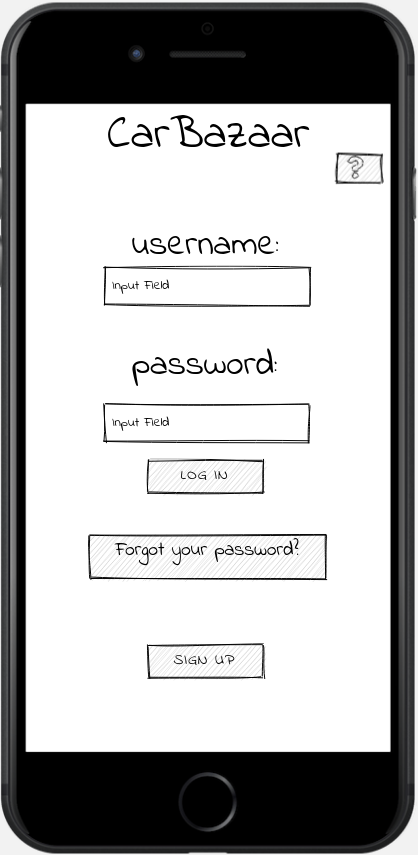
\includegraphics[scale=0.5]{img/wireframes/login_screen.png} }}%
		\qquad
		\subfloat[\centering \en User Dashboard]{{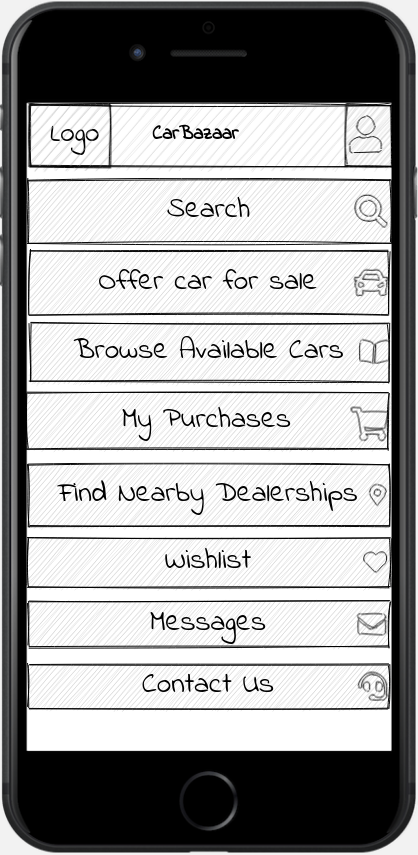
\includegraphics[scale=0.5]{img/wireframes/user_dashboard.png} }}%
	\end{figure}
	
	
	\begin{figure}[htbp!]
		\centering
		
		\subfloat[\centering Αποτελέσματα Αναζήτησης]{{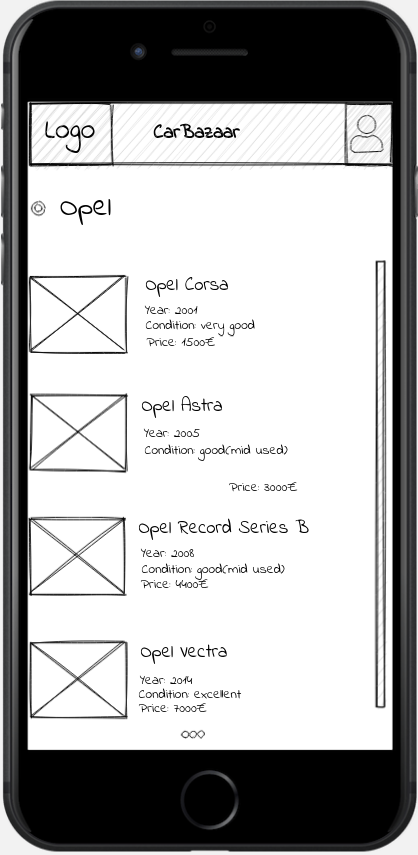
\includegraphics[scale=0.5]{img/wireframes/search_results.png} }}%
		\qquad
		\subfloat[\centering Πληροφορίες Αυτοκινήτου]{{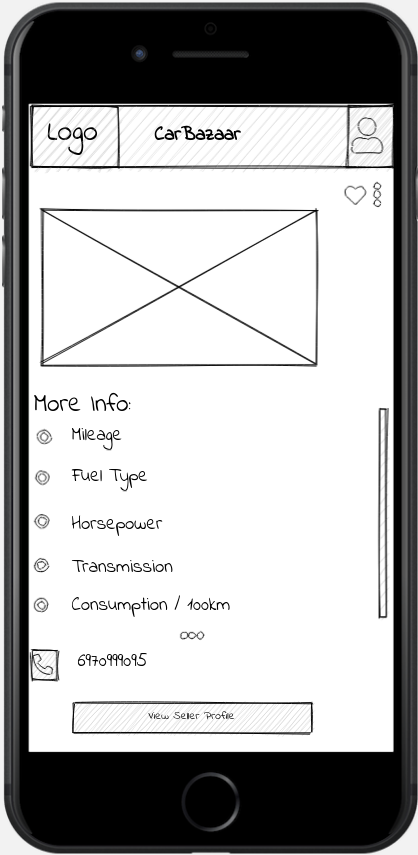
\includegraphics[scale=0.5]{img/wireframes/car_info.png} }}%
		\caption{\en Wireframes \gr για τον χρήστη Πελάτη}%
		
		
	\end{figure}
	
	
	
	
	
	
	
	
	
\end{document}
